\chapter{ISI}

\section{ORACLE APLICATION EXPRESS HR-1}
Oracle Apex adalah platform pengembangan kode rendah yang memungkinkan Anda membangun aplikasi perusahaan yang dapat diskalakan dan aman dengan fitur kelas dunia yang dapat digunakan di mana saja.Oracle apek juga merupakan lingkungan pengembangan perangkat lunak berbasis web yang berjalan pada database Oracle. Ini sepenuhnya didukung dan dilengkapi standar dengan semua edisi Oracle Database dan, dimulai dengan Oracle 11g, diinstal secara default sebagai bagian dari instalasi basis data inti. Data kode rendah pengembangan aplikasi, pertama adalah membuat database, membuat aplikasi, dan menyebarkan aplikasi yang sudah dibuat untuk dipublish. Dalam proses development ini adapula tahapan dalam start, antaralain new. New itu sendiri terdiri atas beberapa bagian antara lain markdown, model,SQL IDE,DML script, dan exel. Dalam proses tersebut maka akan dilakukan proses pengimputan data sql ke database. Selanjutnya akan di exiting menjadi aplikasi yang akan dibangun lalu aplikasi akan dites sebelum memasuki proses produksi pembuatan aplikasi. 
\begin{figure}[!htbp]
    \centering
    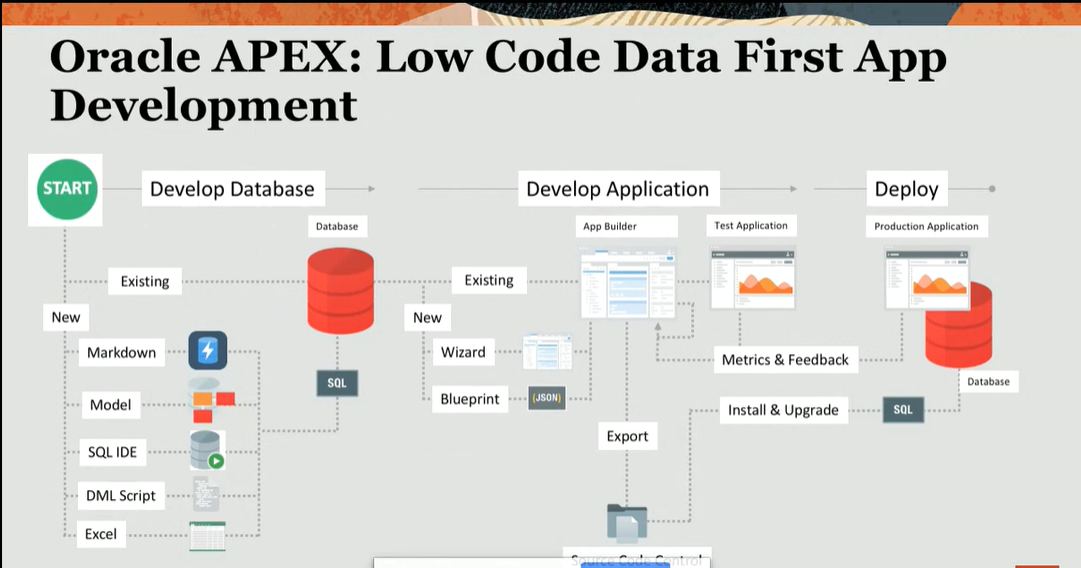
\includegraphics[scale=0.65]{section/hiya.PNG}
    \caption{Proses pembuatan aplikasi pada oracle apex}
    \label{gambar 1}
\end{figure}

Oracle Apex juga menyediakan beberapa fitur yang dapat kita gunakan, yaitu:
\begin{enumerate}
    \item Drag and Drop file XLS, CSV, XML, dan JSON.
    Maksudnya, disini kita dipermudah dengan fitur ini karena kita dapat membuat aplikasi hanya dengan "drag and drop" atau geser dan lepas, namun file tersebut harus berekstensi XLS, CSV, XML, ataupun JSON.
    \item Membuat table di Basis Data otonom.
    Oracle Apex sendiri menyediakan Database Otonom, yaitu Database yang memudahkan kita dimana manajemen database, infrastruktur, pemantauan, dan tuning menjadi otomatis. Walaupun admin masih diperlukan namun hal ini dapat mengurangi biaya admin. Jadi kita disini membuat langsung tabel baru di database yang sudah disediakan. 
    \item Mengupload data ke tabel baru.
    Selain bisa mengupload kita juga bisa mengupload table yang sudah kita buat sebelumnya ke Oracle Apex ini
    \item Membuat Aplikasi berdasarkan tabel yang baru dibuat.
    Dan yang paling kerennya kita bisa buat aplikasi secara langsung dan mudah menggunakan tabel yang sudah ada di Oracle Apex.
\end{enumerate}

Mengelola data spreadsheet sangat menantang antaralain
  \begin{enumerate}
      \item Validasi data    \-- manual dan rawan error
      \item Integritas data  \-- tidak menjamin keakuratan data dalam lingkungan multiuser
      \item Keamanan data    \-- penguncian sel tidak efektif
      \item Berbagi data     \-- exel lamban dan sulit utuk dibagikan
  \end{enumerate}  
  
  Mengubah spreadsheet menjadi aplikasi web
  \begin{enumerate}
      \item Sign in apex.oracle.com
      \item Membuat workspace
      \item Buka app builder >create a new app>  drag dan drop file> pilih movie > next
      \item Isi pada table nama, serta jenis huruf yang digunakan
      \item Setelah itu create application lalu akan memasuki appreance yang dimana berisikan jenis- jenis tabel yang ada, pilih icon sesuai keinginan. pada feature centang semua kolom
      \item Run aplikasi dengan memasukan kata sandi dan username
      
  \end{enumerate}
\par
Database centric framework pengembangan aplikasi web antara lain mengembangkan aplikasi web desktop dan seluler, memvisualisasikan dan memelihara data basis data, meningkatkan keterampilan sql dan kemampuan basis data. aplikasi  yang cocok dengan oracle apex antara lain aplikasi  yang kritis  memilikinmisi besar untuk ribuan pengguna, mengisi kekosongan dalam sistem perusahaan, proses bisnis kedaluwarsa steamline, modernisasi sistem lama, mengganti spreadsheet. 



\section{Tahapan Pembuatan Aplikasi Oracle Apex}
Langkah pertama yang harus dilakukan adalah membuka website https://apex.oracle.com, disini kita akan mendapatkan akses untuk memasuki Oracle Apllication Express, pastikan email yang dimasukkan valid untuk membuat Workspace, berikut adalah langkah langkah pembuatan Aplikasi pada Oracle APEX :

\begin{enumerate}
\item Pergi ke Website Oracle APEX, https://apex.oracle.com, lalu klik tombol \textit{Get Start For Free} di pojok kanan atas.
    
\item Lalu akan muncul tombol \textit{Request a Free Worksace} dan klik tombol tersebut.

\item Isikan data diri anda seperti nama,email,dan workspace.
        
\item Centang apakah anda pernah melakukan hal tersebut lalu next.
      
\item Isikan pada kolom tersebut bebas, mengapa anda ingin menggunakan layanan ini ?, lalu klik next.
 
\item Centang Accept, lalu klik next.

\item Tahapan terakhir untuk mengkonfirmasi apakah ini anda, lalu klik next.

\item Setelah Workspace Sukses Dibuat akan muncul tampilan bahwa Workspace berhasil dibuat dan anda disuruh untuk mengecek email anda.

\item Setelah Workspace baru telah dibuat lanjutkan dengan klik \textit{Continue to sign in screen}.

\item Sign dengan akun anda dengan menginputkan project, username, dan password.


\item Sekarang kita masuk ke tampilan halaman awal aplikasi Oracle Express.

\begin{figure}
\item Buka App Builder lalu klik Create New App.

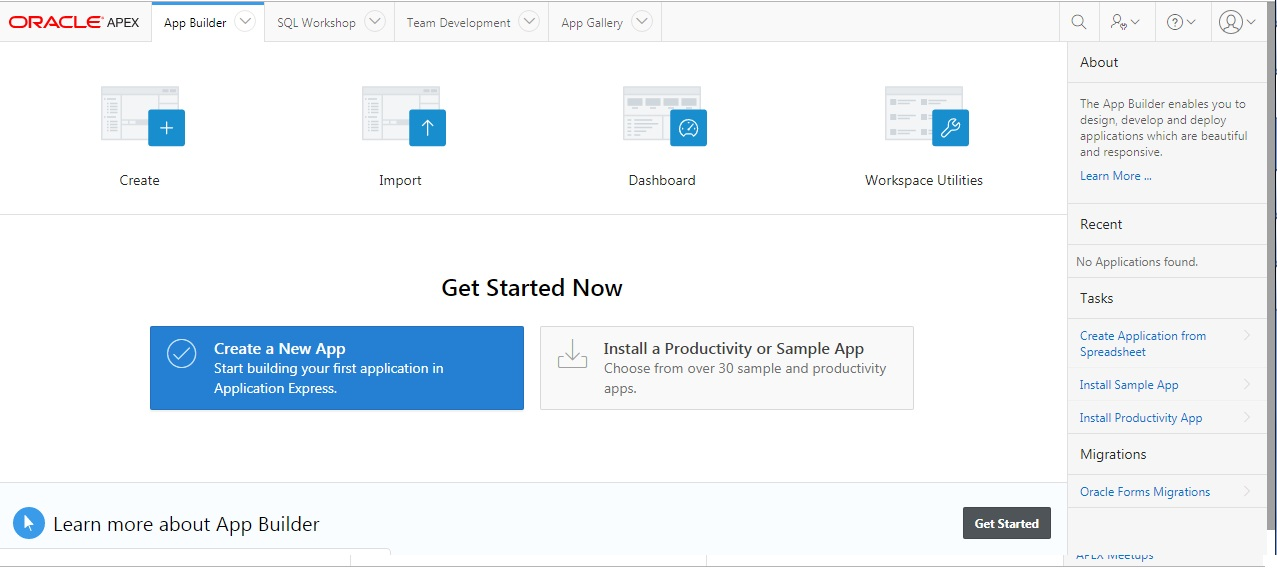
\includegraphics[scale=0.4]{figure/pict(8).jpg}
    \caption{\textit{Oracle Apex App Builder}}
\label{gambar}
\end{figure}

\begin{figure}
\item Klik Copy and Paste, pada select data CSV atau Sample Data Set pilih Project and Tables lalu next.

    \begin{center}
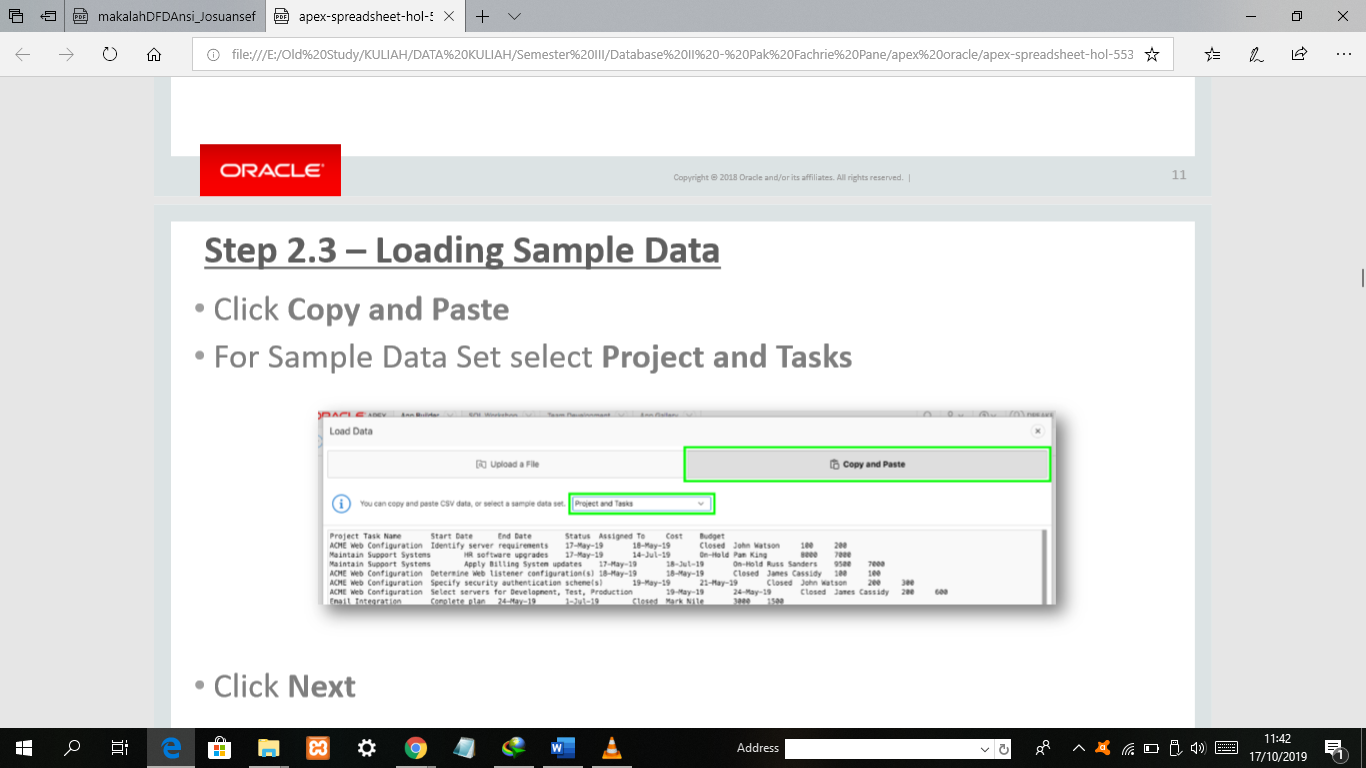
\includegraphics[scale=0.2]{figure/pict(9).png}
    \caption{\textit{Sample Data Set/ Select data CSV}}
        \end{center}
\label{gambar}
\end{figure}

\begin{figure}
\item Setelah Sudah me-Load data, tampilan selanjutnya akan seperti berikut. masukkan nama tabel {SPREADSHEET}, table owner, error Table Name dan Primary Keys, lalu klik load data

    \begin{center}
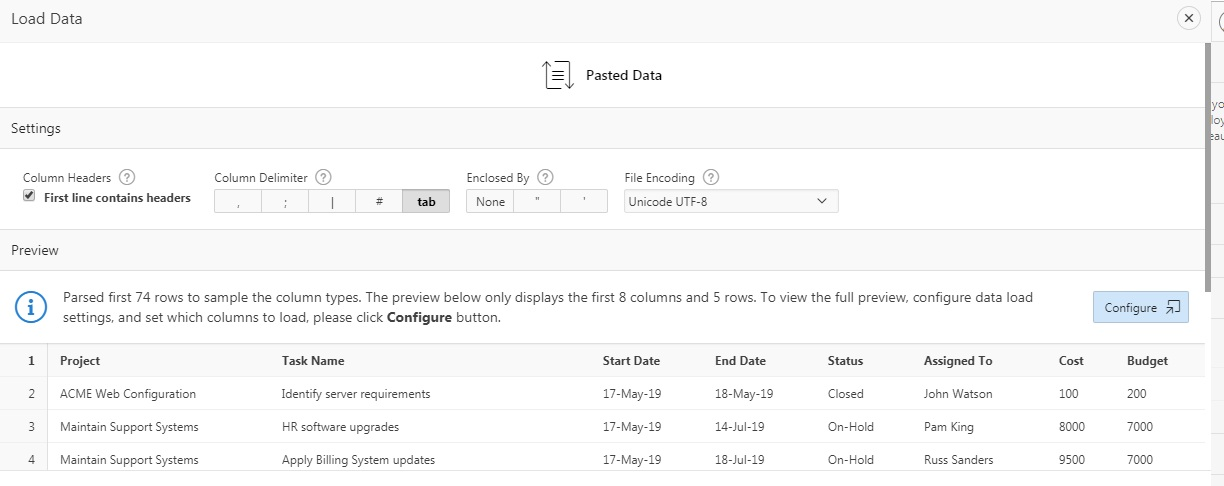
\includegraphics[scale=0.4]{figure/pict(10).jpg}
    \caption{\textit{Load Data.}}
        \end{center}
\label{gambar}
\end{figure}

\begin{figure}
    \begin{center}
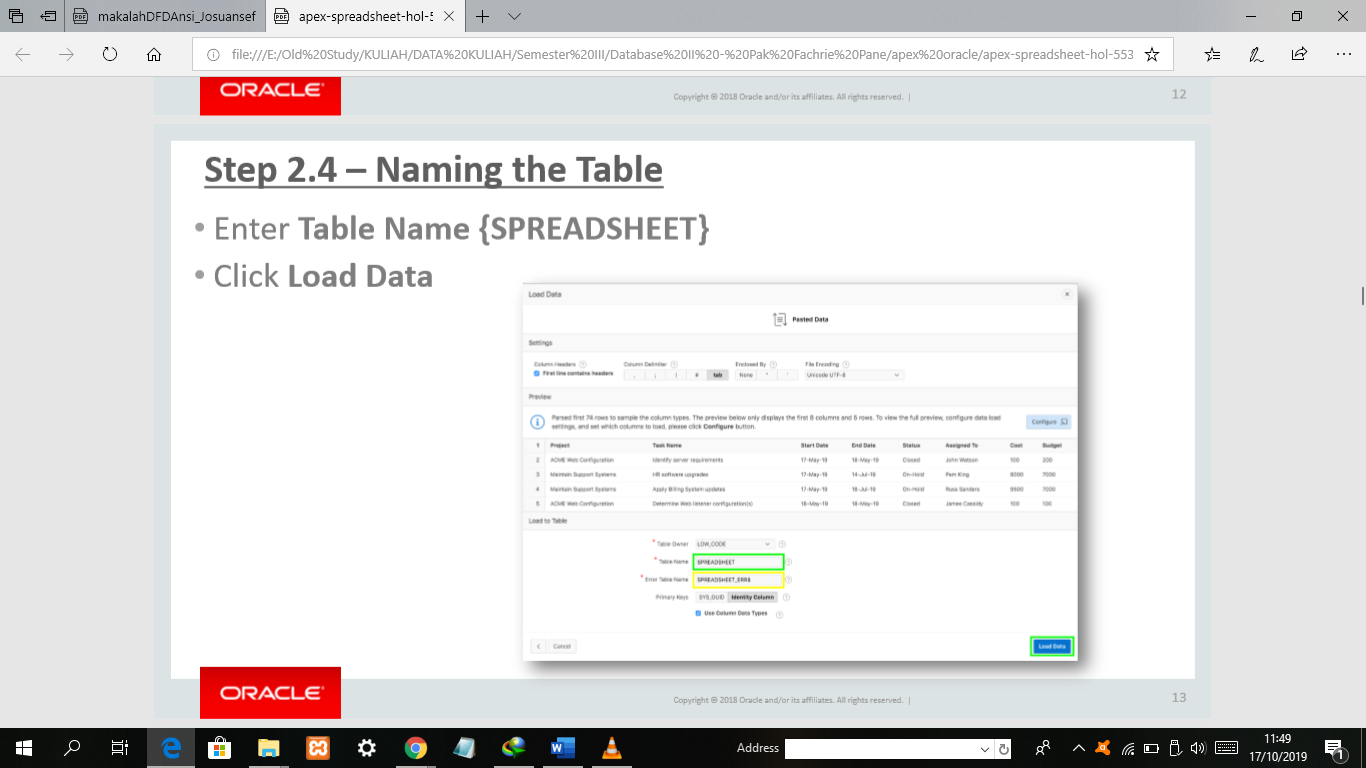
\includegraphics[scale=0.2]{figure/pict(11).png}
    \caption{\textit{Load Data 2}}
        \end{center}
\label{gambar}
\end{figure}

\begin{figure}
\item Load Data Sukses , klik Continue to Create Aplication Wizard.

    \begin{center}
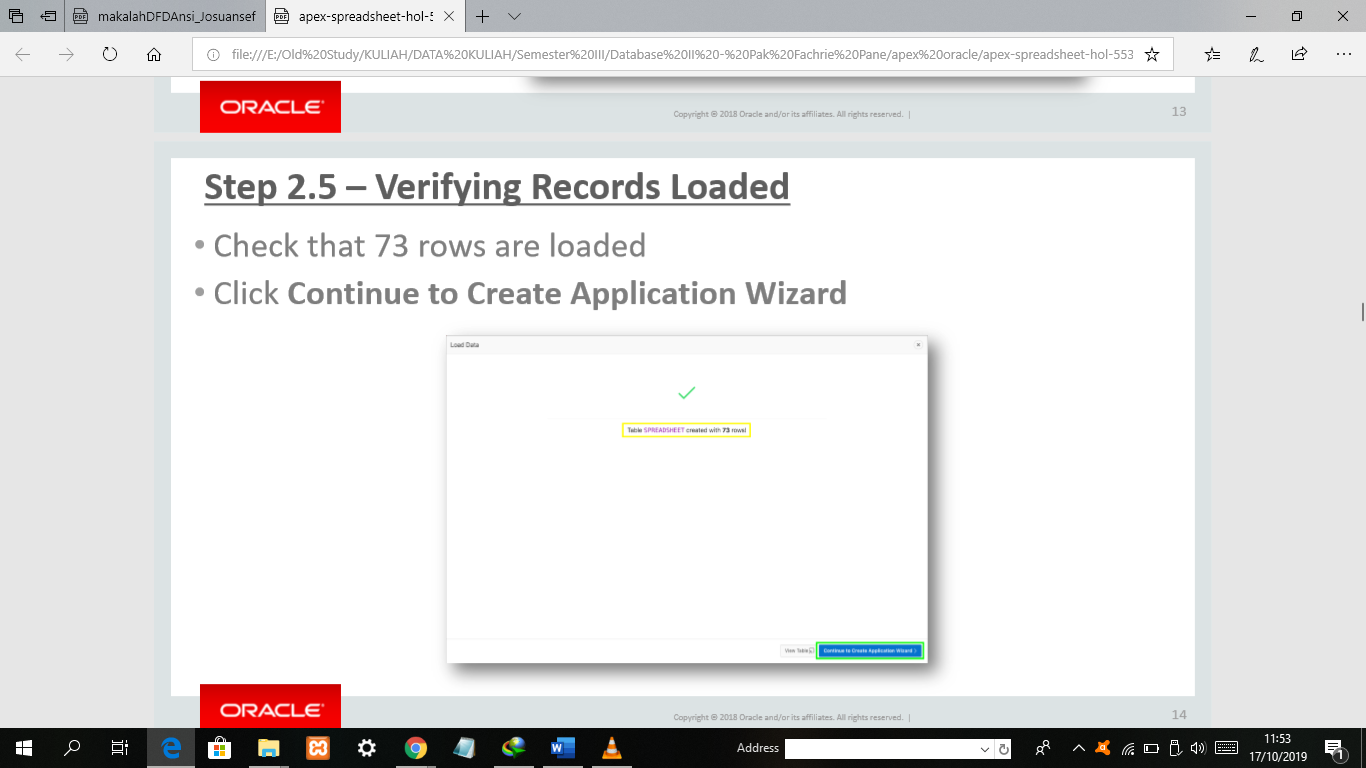
\includegraphics[scale=0.2]{figure/pict(12).png}
    \caption{\textit{Oracle Apex Load Data Success.}}
        \end{center}
\label{gambar}
\end{figure}

\begin{figure}
\item Sekarang kita berada di tampilan Create an Aplication, ikuti langkah berikut, buat nama App from a Spreadsheet lalu pada Features klik Check All.

    \begin{center}
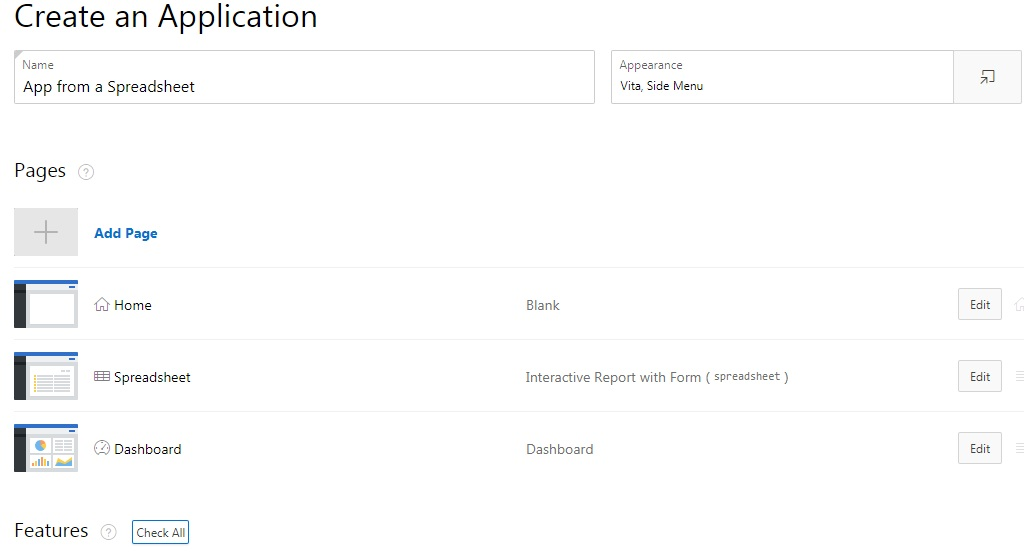
\includegraphics[scale=0.4]{figure/create1.jpg}
    \caption{\textit{Create an Aplication.}}
        \end{center}
\label{gambar}
\end{figure}


\begin{figure}
\item Scroll ke bawah lalu klik Create Application .

    \begin{center}
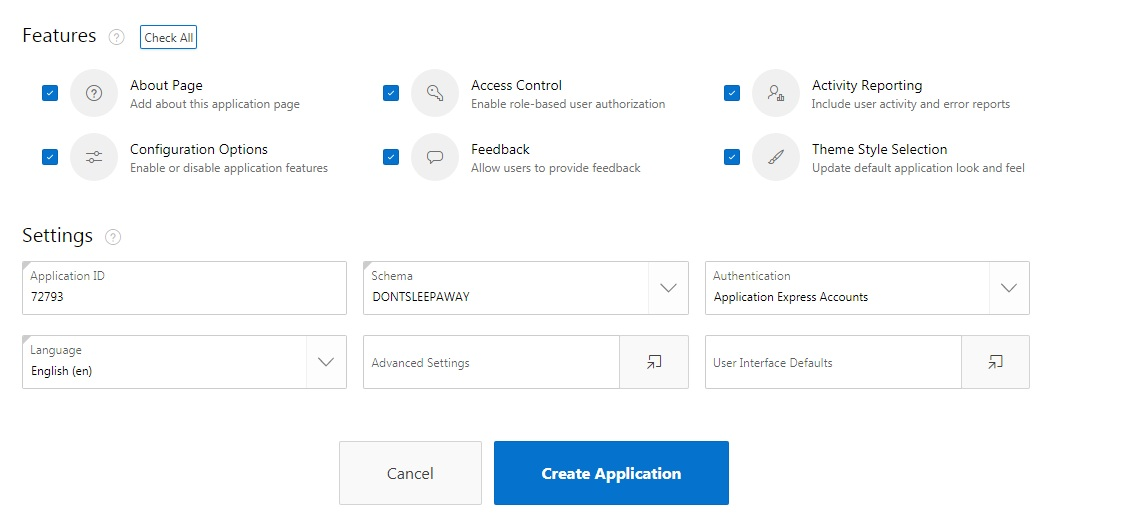
\includegraphics[scale=0.4]{figure/create2.jpg}
    \caption{\textit{Create an Application}}
        \end{center}
\label{gambar}
\end{figure}

\begin{figure}
\item Tunggu beberapa saat selamat data sedang dimuat.

    \begin{center}
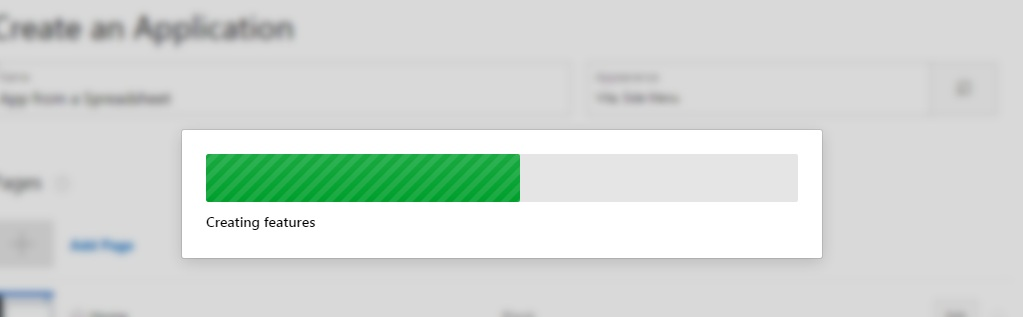
\includegraphics[scale=0.4]{figure/create3.jpg}
    \caption{\textit{Loading Data}}
        \end{center}
\label{gambar}
\end{figure}

\begin{figure}
\item Sekarang kita masuk ke halaman App Builder project Spreadsheet yang telah berhasil dibuat. aplikasi yang baru dibuat akan tampil di halaman designer, setelah itu klik Run application .

    \begin{center}
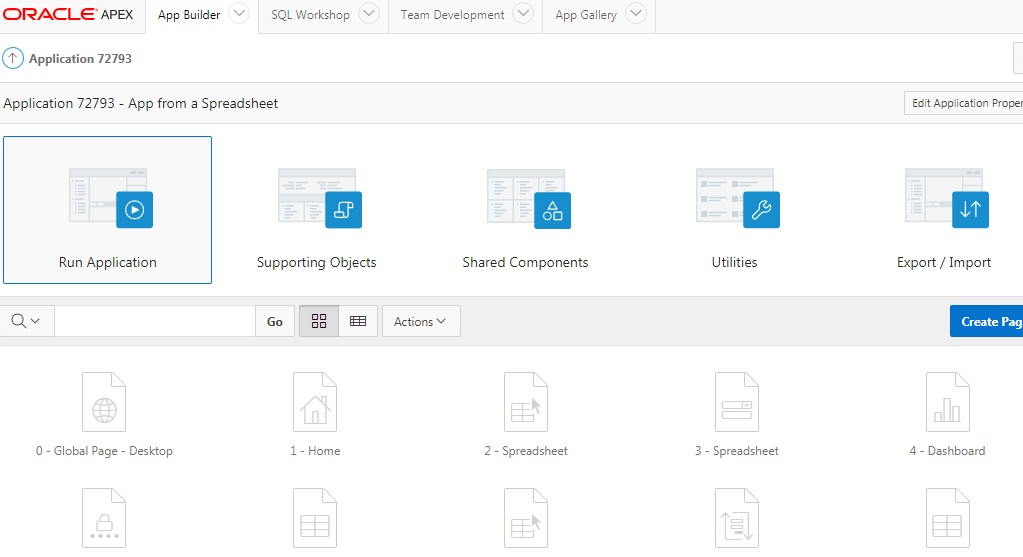
\includegraphics[scale=0.4]{figure/create4.jpg}
    \caption{\textit{App Builder Success}}
        \end{center}
\label{gambar}
\end{figure}

\begin{figure}
\item Login ke Aplikasi yang baru dibuat tadi dengan menggunakan login Oracle APEX .

    \begin{center}
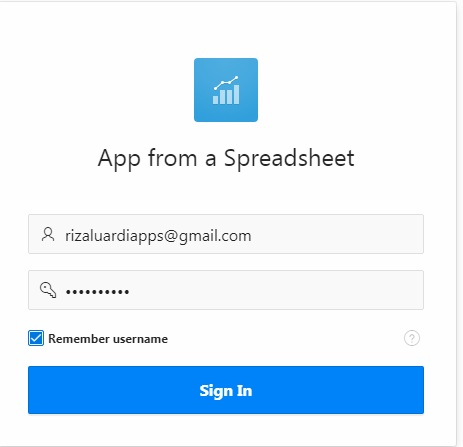
\includegraphics[scale=0.4]{figure/create5.jpg}
    \caption{\textit{Sign In Spreadsheet}}
        \end{center}
\label{gambar}
\end{figure}

\begin{figure}
\item Sekarang aplikasi Oracle Apex sudah dijalankan.

    \begin{center}
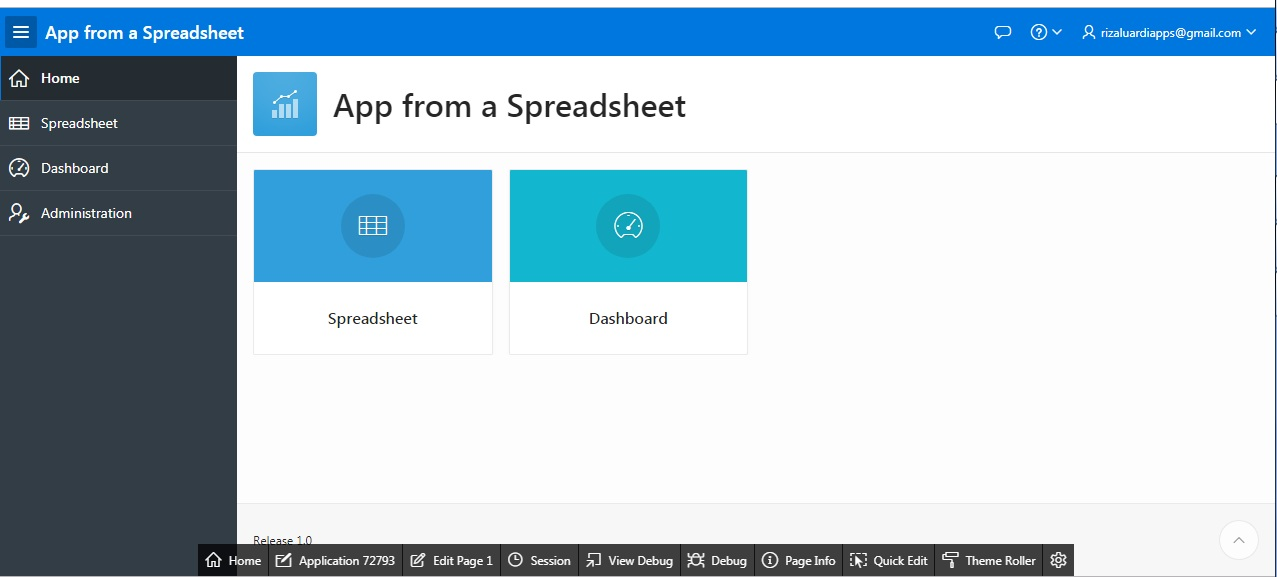
\includegraphics[scale=0.4]{figure/congratz.jpg}
    \caption{\textit{Welcome Spreadsheet}}
        \end{center}
\label{gambar}
\end{figure}

\end{enumerate}

 